\chapterimage{Pictures/Ausberto/2_planejamento.png} % Table of contents heading image
\begin{comment}
    Prof. Dr. Ausberto S. Castro Vera
    UENF - CCT - LCMAT - Curso de Ciência da Computação
    Campos, RJ,  2022
    Disciplina: Análise e Projeto de Sistemas
    Aluno: João Vítor Fernandes Dias
\end{comment}

\chapter{Etapa de Planejamento}
    Neste capítulo é apresentado toda a estrutura de planejamento do projeto, passando por tópicos como Solicitação do sistema, Benefícios e estudo de viabilidade.

    \section{Solicitação do Sistema}
    
    Abaixo serão apresentadas maiores explicações sobre o sistema proposto e suas especificidades.
    
    
        \subsection{Responsável}
            % (o título do cargo): Pessoa que vai estar dentro da empresa e responsável pelo gerenciamento do sistema.
            João Vítor Fernandes Dias   % Analista de sistemas
            
        \subsection{Necessidade da empresa}
            % (É a justificativa/motivo relacionado a atividade empresarial do sistema):
            Este projeto de desenvolvimento de sistema tem como foco a otimização da dinâmica burocrática necessária aos trâmites internos de uma instituição acadêmica, bem como a melhoria do bem estar dos alunos e funcionários ao adicionar novas funcionalidades ao sistema acadêmico anterior. Isso se dando através de maior facilidade de acesso, manipulação e divulgação dos dados.
        
        \subsection{Requisitos de negócios}
            % Quais serão as capacidades do negócio
            \begin{itemize}
                \item Disponibilizar o quadro de horários aos alunos
                \item Disponibilizar os documentos e formulários para que possam ser preenchidos e encaminhados online
                \item Estruturar dados que serão expostos visualmente em formato gráfico em relação às estatísticas envolvendo os cursos
                \item Fornecer aos alunos e funcionários o acesso online às informações acadêmicas
                \item Permitir que coordenadores manipulem as turmas e os alunos
                \item Permitir que coordenadores possam analisar as demandas de matérias
                \item Permitir que os professores manipulem seu quadro de horários
                \item Viabilizar o acesso aos extratos acadêmicos dos alunos
            \end{itemize}
            
        \subsection{Valor agregado}
            % (As vantagens que o sistema trará a organização)
            \begin{itemize}
                \item Economia de custos em artigos de papelaria por causa da redução de documentos físicos
                \item Lucro pela venda do sistema antigo a outras instituições
                \item Melhoria da satisfação dos alunos e funcionários para com a instituição
                \item Potencial aumento de velocidade nos trâmites burocrático
                \item Redução do volume de estoque dos documentos físicos
                \item Redução na quantidade de funcionários necessários para gerir as diversas áreas da instituição pois serão automatizadas
            \end{itemize}
            
        \subsection{Outras informações}
        
            \begin{itemize}
                \item Apresentar o novo sistema acadêmico e todas as suas funcionalidades publicamente e obrigatoriamente para todos os funcionários para que todos saibam quais funcionalidades podem utilizar
                \item Finalizar o projeto durante o semestre acadêmico para que testes sejam efetuados o quanto antes, assim evitando que problemas sérios sejam encontrados durante o período crucial de inclusão de matérias
                \item Necessidade de bom domínio da tecnologia utilizada pelos desenvolvedores para evitar brechas de segurança
                \item Por se tratar de um sistema novo, é adequado que existam tutoriais bem detalhados para os antigos e novos usuários do sistema para que se adéquem sem muito esforço ao novo sistema proposto
                \item Proteção rigorosa dos dados privados manipulados pelo sistema por se tratar de informações pessoais dos alunos
            \end{itemize}

%%%%%%%%%%%%%%%%%%%%%%%%%%%%%%%%%%%%%%%%%%%%%%%%%%%%%%%%%
    
    \section{Custos: Desenvolvimento e Operacional} % 27/03/22 - 21h04
        \begin{itemize}
            \item Desenvolvimento
                \begin{itemize}
                    \item Compra dos materiais necessários para o funcionamento do sistema
                    \item Custos diários com materiais de limpeza e alimentação
                    \item Salário dos desenvolvedores e gestores do projeto
                \end{itemize}
            \item Operacional
                \begin{itemize}
                    \item Aquisição dos softwares proprietários
                    \item Custo do consumo de energia elétrica, água e internet
                    \item Gastos necessários para a mudança do sistema
                    \item Manutenção dos equipamentos
                    \item Salário da equipe operacional % O que é uma equipe operacional?
                \end{itemize}
        \end{itemize}
        
    \section{Benefícios}    % 27/03/22 - 21h24
    
        Essa seção listará os diversos benefícios que o sistema proposto trará. Esses benefícios podem ser divididos em Tangíveis e Intangíveis, como vê-se a seguir.
        
        \subsection{Tangíveis}
            \begin{itemize}
                \item Aumento do uso da plataforma acadêmica pelos alunos e funcionários
                \item Disponibilização de todo o conteúdo das aulas online
                \item Maior simplicidade na hora de gerir as turmas
                \item Mais facilidade na hora de conferir as matérias disponíveis e os horários conflituosos
                \item Melhor comunicação entre alunos e professores
                \item Redução de travamentos em horários de pico
                \item Utilização relevante durante todo o semestre letivo
            \end{itemize}
    
        \subsection{Intangíveis}
            \begin{itemize}
                \item Maior satisfação dos estudantes e professores
                \item Maior transparência em relação às notas e atividades ofertadas
                \item Mais disponibilização de informação aos estudantes
                \item Menos estresse para os coordenadores
                \item Sistema acadêmico exemplar em relação às outras instituições de ensino
            \end{itemize}
    % \section{Análise de Custos e Benefícios}    % 27/03/22 - 21h35 - não fiz
    
    \section{Estudo de Viabilidade}    % 27/03/22 - 21h48
        Aqui daremos mais informações sobre o projeto em si, e com essas informações chegaremos a conclusão quanto a sua viabilidade.
        
        \subsection{Calendário}    % 27/03/22 - 21h50
            \begin{itemize}
                \item Início do projeto: 01/07/2022
                \item Planejamento:      01/07/2022 - 01/09/2022
                \item Análise:           01/09/2022 - 01/11/2022
                \item Projeto:           01/11/2022 - 01/01/2023
                \item Implementação:     01/01/2023 - 01/07/2023
                \item Conclusão:         01/07/2023
            \end{itemize}
    
        \subsection{Cronograma}    % 27/03/22 - 22h02
            Com a Figura \ref{cronograma} demonstra-se a dispersão das atividades ao longo do período esperado para desenvolvimento e conclusão do projeto.
            \begin{figure}[htbp]\centering
                \caption{Cronograma de atividades}
                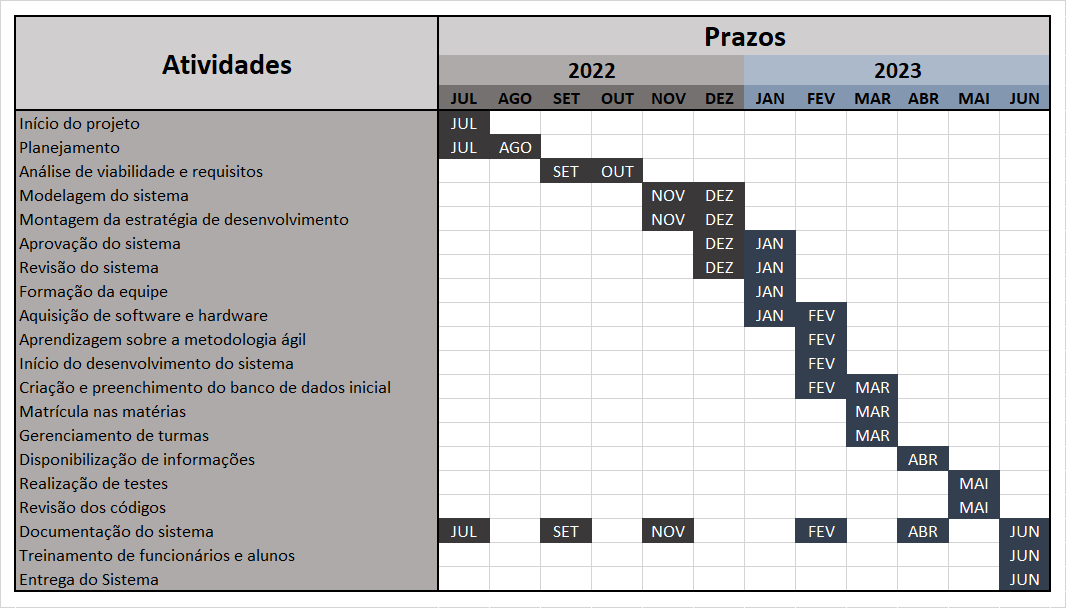
\includegraphics[angle=0,scale=0.68]{Pictures/JV/Cronograma.png}
                \label{cronograma}
            \end{figure}    % IMAGEM CRONOGRAMA DE ATIVIDADES
    
        % \subsection{Alternativas Tecnológicas}  % Não fiz
            % Hardware, Software, Treinamento, etc...
        
        \subsection{Orçamento}  % 27/03/22 - 22h45
            % Considere as Alternativas Tecnológicas para fazer pelo menos 3 orçamentos diferentes
            O orçamento descrito detalhadamente com o custo total e a quantidade de cada componente está ilustrado na Figura \ref{orcamento}.
            \begin{figure}[htbp]\centering
                \caption{Orçamento}
                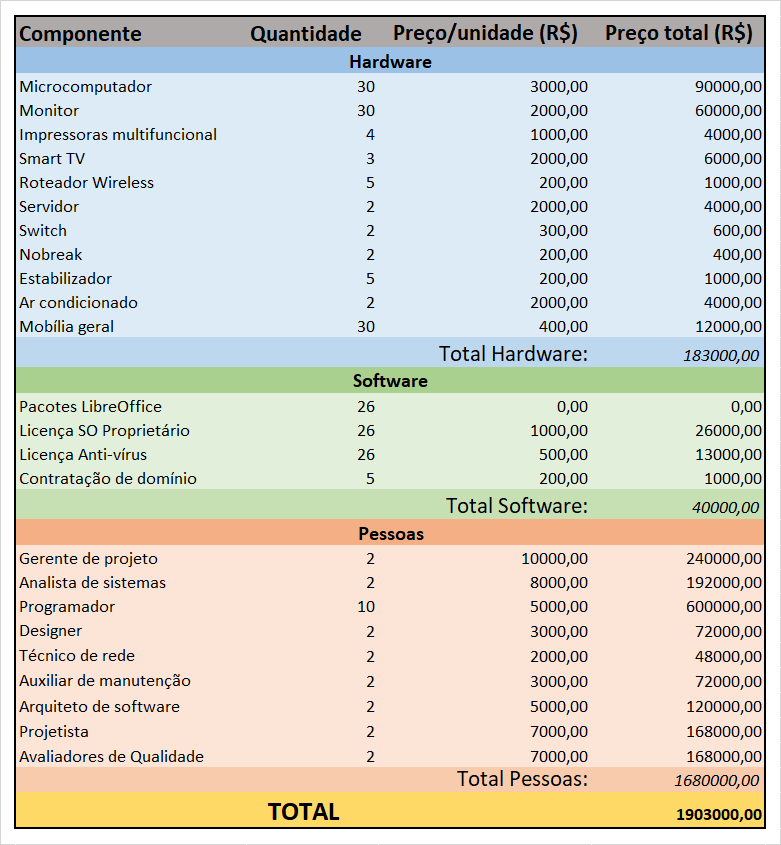
\includegraphics[angle=0,scale=0.68]{Pictures/JV/Orçamento.png}
                \label{orcamento}
            \end{figure}    % IMAGEM ORÇAMENTO
        
        \subsection{Recomendações}
            % [   FALTA FALAR SOBRE TECLADOS E MOUSES ]
        
            É recomendado que os períodos indicados na Figura \ref{cronograma} sejam seguidos, mas entende-se que possam surgir imprevistos, ainda assim, o prazo final precisa ser cumprido. Além disso, é adequado que para se manter dentro do orçamento sejam comprados os item listados no orçamento \ref{orcamento} e contratados funcionários com o salário estipulado. Assim como surgem imprevistos com os prazos, espera-se o surgimento de imprevistos em relação aos equipamentos.
            % Quanto a isso, utiliza-se da verba disponibilizada para imprevistos [ADICIONAR NA TABELA].
        
        \subsection{Resumo}
            Considerando o orçamento disponível e as necessidades do sistema, conclui-se que o desenvolvimento do sistema acadêmico é viável.